\section{Schnittstellen}
\subsection{Externe Schnittstellen}
Die folgenden externen Schnittstellen sind im Projekt enthalten:
\begin{enumerate}
	\item Logger
	\item LoggerSetup
	\item LogLevel
	\item StringPersitor
\end{enumerate}

\subsubsection{Logger}
\begin{figure}[H]
	\centering
	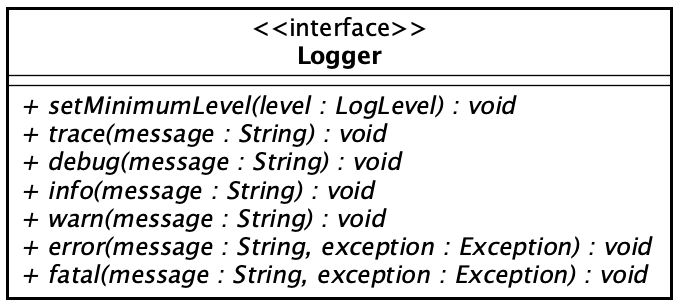
\includegraphics[width=0.5\textwidth]{3_Schnittstellen/Bilder/loggerInterface.png}
	\caption{LoggerInterface Klassendiagram}
	\label{fig:LoggerInterface Klassendiagramm}
\end{figure}
Das Logger-Interface, über welches verschiedenste Applikationen Log-Einträge erfassen können enthält insgesamt acht Methoden. Für die einzelnen Log-Levels existieren eigene Methoden. Des Weiteren enthält das Logger-Interface eine Methode zur Setzung des minimalen Log-Levels. 
\subsubsection{LoggerSetup}
\subsubsection{LogLevel}
\subsubsection{StringPersistor}

\subsection{Interne Schnittstellen}
Die folgenden internen Schnittstellen wurden durch das Projektteam definiert: 
\begin{enumerate}
	\item LogMessage
	\item LogPersistor
	\item TCP / IP
	\item client.properties
	\item server.properties
\end{enumerate}

\subsubsection{LogMessage}
\subsubsection{LogPersistor}
\subsubsection{TCP / IP}
\subsubsection{client.properties}
\subsubsection{server.properties}